% !TeX program = lualatex
% !TeX root = luaking.tex
% !TeX encoding = UTF-8
% !TeX spellcheck = cs_CZ
%---------------------------------------------------------------------------------------------------
% file tky1ch02.tex
%---------------------------------------------------------------------------------------------------
%================== Kapitola: LTI systém ===========================================================
\setchaptertoc
\chapter{LTI systém}\label{tky:IchII}
  \twocolumn[\section{Vlastnosti a popis lineárních systému}\label{tky:IchIIsecI}]
    Na soustavu obvodů můžeme nahlížet jako na seskupení (množinu) navzájem souvisejících součástí,
    ke kterému je určen vstupní signál \(x\), zvaný \emph{buzení} a výstupní signál \(y\),
    označovaný jako \emph{odezva}. Z hlediska vlastností jde o systém představující "černou
    skříňku", jejíž vlastnosti můžeme identifikovat analýzou vstupního a výstupního signálu
    \cite{Bicak2007}.   

    \luagraphic[0.8]{tky_fig005.pdf}{Symbol soustavy s jedním vstupem a jedním výstupem}{tky:fig005}

    \begin{description}[leftmargin=3em,labelindent=1em, style=nextline]
      \item[Systémy se spojitým časem] (na vstupu i výstupu pracují se spojitými signály) - relace  
            mezi vstupem a výstupem můžeme symbolicky zapsat:
            \begin{equation}\label{tky:eq005}
              y(t)=S\{x(t)\}
            \end{equation}
            kde \(S\) je obecný popis systémové funkce, přiřazující vstupní veličině \(x(t)\) odezvu 
            \(y(t)\). Z rovnice je zřejmé, že u spojité (analogové) soustavy výstupní signál závisí 
            na všech hodnotách vstupního signálu, nikoli jen na některých jeho hodnotách v určitých 
            časových okamžicích.
            \luagraphic[0.8]{tky_fig015.pdf}{Systém se spojitým časem}{tky:fig015} 
      \item[Systémy pracující s diskrétním časem] lze obdobně symbolicky vyjádřit relací  
            vstup/výstup ve tvaru:
            \begin{equation}\label{tky:eq022}
              y[n]=S\{x[n]\}
            \end{equation}
            kde \(S\) je tentokráte systémový operátor přiřazení posloupnosti \(x[n]\rightarrow
            y[n]\). U diskrétních systémů se zpracovávají posloupnosti hodnot signálů, získaných
            vzorkováním spojitého signálu
            \luagraphic[0.8]{tky_fig016.pdf}{Systém s diskrétním časem}{tky:fig016}     
      \item[Linearita systémů] ve spojité diskrétní oblasti má velký význam, neboť dovoluje využívat
            princip superpozice k zjednodušování úloh jejich analýzy  a syntézy.

            Předpokládejme, že na vstupu lineárního diskrétního systému jsou přivedeny dva signály
            \(x_1[n]\) a \(x_2[n]\). Účinky obou vstupních signálů na výstupní signál lze zkoumat
            odděleně a podle \emph{principu superpozice} je na výstupu sečíst. Označme dílčí odezvy
            \(y_1[n]=S\{x_1[n]\}\) a \(y_2[n]=S\{x_2 [n]\}\), potom je
            \begin{equation}\label{tky:eq007}
              y[n]= y_1[n]+y_2[n]=S\{x_1[n]+x_2[n]\}
            \end{equation}
            Analogický vztah platí i pro lineární spojitý systém, tedy
            \begin{equation}\label{tky:eq008}
              y(t)= y_1(t)+ y_2(t)=S\{x_1(t)+x_2(t)\}
            \end{equation}
            Z uvedeného vyplývá významná vlastnost lineárního systému. \emph{Výstupní spektrum může
            obsahovat pouze ty frekvence, které jsou ve spektru vstupního signálu a žádné jiné.} 

      \item[Systém časově invariantní] je charakterizován tím, že události jsou v čase závislé pouze
            na časovém intervalu (rozdílu časových událostí), nikoliv na každém časovém okamžiku
            samostatně. Systém je časově invariantní, jestliže časový posun ve vstupní signálu vede
            ke stejnému posunu výstupního signálu. Odezva diskrétního systému na posunutý vstupní
            signál \(x[n-m]\) je pak určen vztahem
            \begin{equation}\label{tky:eq009}
              y[n-m]= S\{x[n-m]\}
            \end{equation}
            a obdobně pro odezvu spojité soustavy na posunutý (zpožděný) vstupní signál
            \(x(t-\tau)\) platí analogicky rovnice
            \begin{equation}\label{tky:eq010}
              y(t-\tau)= S\{x(t-\tau)\}.
            \end{equation}
    \end{description}

    Takový systém má konstantní parametry a je popsaný \emph{diferenčními rovnicemi s konstantními
    koeficienty}. 
    
    Zcela obecně se \textsc{LTI} systém vyznačuje ještě dalšími vlastnostmi, z nichž jsou pro
    analýzu významnější kauzalita a stabilita. 
    \begin{description}[leftmargin=3em,labelindent=1em, style=nextline]
      \item[Kauzální, příčinný systém] - výstupní signál závisí pouze na současných a
            minulých hodnotách vstupního signálu \(x[n]\), nikoliv na budoucích hodnotách, nikoliv
            na budoucích hodnotách. Nicméně existují významné struktury (např. filtry), při jejichž
            návrhu vycházíme z vlastností nerealizovatelné - ideální struktury, které vhodnou
            metodou aproximace vyjádříme realizovatelnou strukturou. U \textsc{LTI} systémů může být
            otázka kauzality převedena na vlastnosti impulzní odezvy - viz. odst.
            \ref{tky:IchIIsecIssecII}. Při uložení signálu do paměti lze realizovat i nekauzální
            systém, který ale nepracuje v reálném čase. 
      \item[Stabilní systém] - omezený vstup (v hodnotách) produkuje též omezený výstup.
            Jinak - není-li vstup divergentní, pak ani výstup nebude divergentní. Uvedené bude
            splněno, jestliže pro hodnoty impulzní odezvy \(h[n]\) bude platit
            \begin{equation*}
              \sum_{n=-\infty}^\infty\abs{h[n]} <\infty.
            \end{equation*}
            Problém stability se vyskytuje u rekurzivních struktur (struktury se zpětnou vazbou). 
    \end{description}      

    \subsection{Konvoluce v diskrétních systémech}\label{tky:IchIIsecIssecII}
      Významnou charakteristikou lineárních časově invariantních systémů \textsc{LTI} je
      \textbf{impulsní odezva}. Její znalost umožňuje stanovit odezvu systému na obecný signál, lze 
      ji využít i při syntéze systému \cite{Bicak2007}.

      Mějme diskrétní \textsc{LTI} systém \ref{tky:fig002}, na jehož vstup je přiveden
      \emph{jednotkový diskrétní impuls}\footnote{Nesmíme zaměňovat s Diracovým (také jednotkovým)
      impulsem.}. Jednotkový impuls je posloupnost \(\delta[n]=0\) pro všechna \(n\) s výjimkou
      \(\delta[0]=1\). Odezva systému na jednotkový impuls \(\delta[n]\) se nazývá impulsní odezva a
      platí
      \begin{equation}\label{tky:eq011}
        h[n]= S\{\delta[n]\}.
      \end{equation}
      Vzhledem časové invariantnosti, posunutému jednotkovému impulsu odpovídá posunutá impulsní
      odezva, tedy
      \begin{equation}\label{tky:eq012}
        h[n-m]= S\{\delta[n-m]\}.
      \end{equation}
      \emph{Jednotkový skok} \(1[n]\) je posloupnost jedniček od počátku časové osy \(n=0\),
      kterou můžeme zapsat součtem
      \begin{align}
        1[n]&= \sum_{m=0}^n\delta[n-m]                  \nonumber \\
            &=\delta[n]+\delta[n-1]+\delta[n-2]+\cdots. \label{tky:eq013}
      \end{align}
      \emph{Odezva systému na jednotkový skok} $\mathrm{1}[n]$ se nazývá \textbf{přechodová odezva}
      $s[n]$ a platí
      \begin{align}
        s[n]&= S\{1[n]\}= S\{\sum_{m=0}^n\delta[n-m]\}        \nonumber \\
            &=\sum_{m=0}^nS\{\delta[n-m]\}.                             \label{tky:eq014}
      \end{align}

      Postupná úprava rovnice (\ref{tky:eq014}) je umožněna díky linearitě systému, kterou budeme
      studovat pro obecný vstupní signál
      \begin{equation}\label{tky:eq015}
        x[n]=\sum_{m=-\infty}^\infty x[m]\delta[n-m].
      \end{equation}
      Poznamenejme, že formou (\ref{tky:eq015}) lze zapsat každý diskrétní signál.

      \begin{figure}[ht!]
        \centering  
        \subcaptionbox{\label{tky:fig_006a}}{\luafigure[0.45]{tky_fig006a.pdf}}
        \subcaptionbox{\label{tky:fig_006b}}{\luafigure[0.45]{tky_fig006b.pdf}}
        \caption{Posloupnost jednotkového skoku a) \(1[n]\) a b) signálu \(x[n]\)}
        \label{tky:fig_006}
      \end{figure}

      Na obr. \ref{tky:fig_006} je znázorněna souvislost mezi posloupností jedniček a diskrétním
      signálem. \emph{Posloupnost jedniček tvoří bázi pro diskrétní signály}. Každá komponenta
      diskrétního signálu je vyjádřena součinem $x[m]\delta[n-m]$. V uvedeném příkladě jde o
      posloupnost příslušnou jednotkovému skoku
      \begin{equation*}
        1[n]=\sum_{m=0}^{15}\delta[n-m]
      \end{equation*}
      a odpovídající posloupnost konečného signálu
      \begin{equation*}
        x[n]=\sum_{m=0}^{15}x[m]\delta[n-m].
      \end{equation*}

      \begin{figure*}[ht!]
        \centering
        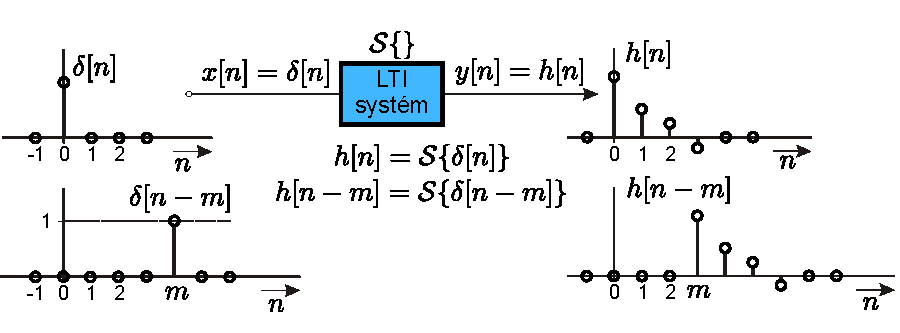
\includegraphics[scale=0.9]{tky_fig002.pdf}
         \caption[impulsní odezva]{Odezva kauzálního diskrétního systému na jednotkový impuls
                  $\delta[n]$ a posunutý impuls $\delta[n-m]$}
        \label{tky:fig002}
      \end{figure*}

      Princip superpozice dovoluje získat odezvu systému jako sumu odezev na jednotlivé dílčí
      součásti vstupního signálu, které v rovnici (\ref{tky:eq015}) tvoří vážené jednotlivé impulsy,
      ze kterých je signál složen
      \begin{align}
        y[n]=S\{x[n]\}
          &=S\{\sum_{m=-\infty}^{\infty}x[m]\delta[n-m]\}  \nonumber \\
          &=\sum_{m=-\infty}^{\infty}x[m]S\{\delta[n-m]\}. \label{tky:eq016}
      \end{align}
      Protože platí (\ref{tky:eq011}) a v důsledku časové invariance vyplývá z rovnice
      \ref{tky:eq016} \textbf{konvoluční suma} 
      \begin{align}
        y[n]&=\sum_{m=-\infty}^{\infty}h[n-m]x[m]               \nonumber \\
            &=\sum_{k=-\infty}^{\infty}h[k]x[n-k].              \label{tky:eq017}
      \end{align}
      Uvedli jsme, že u kauzálního systému závisí výstupní signál $y[n]$ pouze na současných a
      minulých hodnotách vstupního signálu $x[n], x[n-1], x[n-2], \cdots ,$ takže v konvoluční sumě
      \ref{tky:eq017}
      \begin{align*}
        y[n]&=\sum_{k=-\infty}^{\infty}h[k]x[n-k]              \\               
            &=\sum_{k=-\infty}^{-1}h[k]x[n-k] + \sum_{k=0}^{\infty}h[k]x[n-k]  
      \end{align*}
      musíme položit všechny členy impulsní odezvy $h[k]=0$ pro $k<0$. Konvoluční suma pro
      lineární, časově invariantní a kauzální systém má pak tvar
      \begin{equation}\label{tky:eq018}
        y[n]=\sum_{k=0}^{\infty}h[k]x[n-k].
      \end{equation}
      Jestliže navíc budeme uvažovat vstupní a výstupní signály, které jsou nulové pro $n<0$ a
      $x[n]\neq0, y[n]\neq0$ pouze pro $n\geq0$, potom platí
      \begin{equation}\label{tky:eq019}
        \boxed{y[n]=\sum_{k=0}^{n}h[k]x[n-k].\,}
      \end{equation}
      nebo
      \begin{equation}\label{tky:eq024}
        \boxed{y[n]=\sum_{k=0}^{n}x[k]h[n-k].\,}
      \end{equation}
      kde \(n\) je pořadový index právě počítaného vzorku výstupní posloupnosti a \(k\) je pořadový
      index vstupní posloupnosti. Je-li délka vstupní posloupnosti \(N_x\) a délka impulzní odezvy
      \(N_h\), pak délka výstupní posloupnosti (počet jejich vzorků) je dána vztahem:
      \begin{equation}\label{tky:eq025}
        N_y = N_x + N_h - 1.
      \end{equation}
      Rovnice \ref{tky:eq019} a \ref{tky:eq024} určují způsob výpočtu výstupního signálu \textsc{LTI}
      systému. Výstupní signál \(y[n]\) je dán součtem prvků impulsové odezvy a vstupního signálu,
      přičemž buď vstupní signál \ref{tky:eq019} nebo impulsová odezva \ref{tky:eq024} jsou otočeny
      v čase \cite[s.~14]{Davidek1996}.
      
      Symbolicky se tato operace zapisuje 
      \begin{equation}\label{tky:eq026}
        \boxed{y[n] = h[n]*x[n]. \,}
      \end{equation}
      %---------------------------------------------------------------
      % !TeX spellcheck = cs_CZ Lineární obvody a systémy - Jan Bičák  - strana 10 Popis spojitých systémů
%===================================================================================================
\begin{mdframed}[style=mdexam]
  \begin{example}\label{tky:exam001}
    Uvažujme LTI systém, popsaný svou impulzní odezvou: \(h[n] = \{0.45, 1.72, 0.62\}\). Na jeho
    vstupu působí posloupnost \(x[n] = \{2,  0.95\}\). Úkolem  je vypočítat vzorky výstupní
    posloupnosti \(y[n]\).

    \noindent\textbf{Řešení:} Podle (\ref{tky:eq025}) bude délka výstupní posloupnosti \(N_y = 2 + 3
    - 1= 4\) s pořadovými indexy 0 až 3. Pro její výpočet rozepíšeme vztah (\ref{tky:eq024}):
    \begin{align*}
      y[0] &= \sum_{k=0}^0 x[0]h[0] = \num{2}\cdot\num{0.45} = \num{0.9}                   \\
      y[1] &= \sum_{k=0}^1 x[k]h[1-k] = x[0]h[1] + x[1]h[0] =                              \\
           &=  \num{2}\cdot\num{1.72} + \num{0.95}\cdot\num{0.45} = \num{3.8675}           \\
      y[2] &= \sum_{k=0}^2 x[k]h[2-k] =                                                    \\
           &= x[0]h[2] + x[1]h[1] + x[2]h[0] =                                             \\
           &= \num{2}\cdot\num{0.62} + \num{0.95}\cdot\num{1.72} + \num{0}\cdot\num{0.45}  
            = \num{2.8740}                                                                 \\
      y[3] &= \sum_{k=0}^3 x[k]h[3-k] =                                                    \\
           &= x[0]h[3] + x[1]h[2] + x[2]h[1] +  x[3]h[0] =                                 \\
           &= \num{2}\cdot\num{0} + \num{0.95}\cdot\num{0.62} + \num{0}\cdot\num{1.72}
            + \num{0}\cdot\num{0.45} =                                                     \\
           &= \num{0.589} 
    \end{align*} 
    Pro výstupní posloupnost tedy platí:
    \begin{equation*}
      y[n] = \{\num{0.9}, \num{3.8675}, \num{2.8740}, \num{0.589}\}
    \end{equation*}
    Situaci názorně shrnuje obr. \ref{tky:fig011}

    {\centering
      \captionsetup{type=figure}
      \luafigure[1]{tky_fig011.pdf}
      \captionof{figure}{Odezva lineárního číslicového systému na vstupní posloupnost. 
                \cite{Zaplatilek2013}}
      \label{tky:fig011}
    \par}

    V systému \textsc{MATLAB} je vestavěna vnitřní funkce \lstinline[style=luaMatlabText]!conv! pro
    snadný výpočet lineární diskrétní konvoluce, jak dokumentuje výpis \ref{tky:lst001}. Vyzkoušejme
    si, že obrátíme-li pořadí proměnných v příkazu \lstinline[style=luaMatlabText]!conv!, vyjde
    shodný výsledek (komutace symbolů).
  \end{example} 
  \begin{lstlisting}[style=luaMatlabText,gobble=4, label={tky:lst001}]
    h = [0.45, 1.72, 0.62];
    x = [2,  0.95];
    y = conv(x,h)
  \end{lstlisting}

\end{mdframed}
      %---------------------------------------------------------------

    \subsection{Konvoluce ve spojitých systémech}\label{tky:IchIIsecIssecIII}
      Podobně můžeme postupovat i v analogovém případě a odvodit pro lineární časově invariantní
      systém \emph{konvoluční integrál}. Vraťme se k výrazu \ref{tky:eq015} kterým jsme vyjádřili
      libovolný diskrétní signál. Pro případ spojitého signálu vytvořme analogickou formu zápisu
      využívající jednotkový impuls. Průběh obecného spojitého lze podle obr. \ref{tky:fig007}
      aproximovat stupňovitým průběhem, který můžeme vyjádřit jako sumu posunutých (zpožděných)
      impulsů. Výchozí aproximující impuls lze vyjádřit vztahem
      \begin{equation}\label{tky:eq027}
          \delta_\varepsilon(t)  =
            \begin{cases}
               \frac{1}{\varepsilon} & \text{pro } \abs{t} < \frac{\varepsilon}{2},      \\
               0                  & \text{pro } \abs{t} > \frac{\varepsilon}{2} > 0
            \end{cases}
      \end{equation}
      a je znázorněn na obr. \ref{tky:fig007b}. \emph{Jednotkový (Diracův) impuls} 
      má jednotkovou plochu.
      \begin{figure}[ht!]
        \centering
          \subcaptionbox{\label{tky:fig007a}}{\luafigure[0.60]{tky_fig007a.pdf}}                                                  
          \subcaptionbox{\label{tky:fig007b}}{\luafigure[0.27]{tky_fig007b.pdf}}                    
        \caption{a) Aproximace spojitého průběhu signálu, b) K odvození jednotkové impulsní funkce 
        (\cite[s.~7]{Bicak2007})}
        \label{tky:fig007}
      \end{figure}
      Matematicky můžeme Diracovův impuls definovat výrazem
      \begin{equation}\label{tky:eq028}
        \delta_\varepsilon(t) = \lim_{\varepsilon\rightarrow0} \delta_\varepsilon(t).
      \end{equation}
      Aproximaci spojitého průběhu $x(t)$ impulsy \ref{tky:eq027} lze vyjádřit rovnicí
      \begin{equation}\label{tky:eq029}
        x(t)=\sum_{m=-\infty}^\infty x(m\varepsilon)\delta_\varepsilon(t-m\varepsilon)\varepsilon.
      \end{equation}
      Zmenšování šířky impulsů $\varepsilon\rightarrow0$ se chyba aproximace zmenšuje a výraz přejde
      v limitu
      \begin{equation}\label{tky:eq030}
        x(t) = \lim_{\varepsilon\rightarrow0}
               \sum_{m=-\infty}^\infty x(m\varepsilon)\delta_\varepsilon(t-m\varepsilon)\varepsilon.        
      \end{equation}
      V limitě kdy $\varepsilon\rightarrow0$, můžeme sumu nahradit integrálem, dále součin
      $m\varepsilon$ integrační proměnnou $\tau$ a $\varepsilon$ jejím diferenciálem. Obdržíme
      \begin{equation}\label{tky:eq031}
        x(t) = \int_{-\infty}^{\infty}x(\tau)\delta(t-\tau)d\tau .
      \end{equation}
      Vztahem \ref{tky:eq031} jsme spojitý průběh signálu vyjádřili jako sumu
      nekonečného počtu posunutých jednotkových impulsů váženou jeho okamžitými hodnotami.
      Předpokládejme dále, že na vstup lineárního časově invariantního spojitého systému je převeden
      jednotkový (Diracův) impuls a systém vytvoří odezvu $h(t)$. V případě obecného vstupního
      spojitého signálu $x(t)$ aproximovaného vztahem \ref{tky:eq031}, bude odezva
      analogového systému
      \begin{equation}\label{tky:eq032}
        \boxed{y(t) = \int_{-\infty}^{\infty}x(\tau)h(t-\tau)d\tau, \,}
      \end{equation}
      nebo
      \begin{equation}\label{tky:eq033}
        \boxed{y(t) = \int_{-\infty}^{\infty}h(\tau)x(t-\tau)d\tau.\,}
      \end{equation}
      Uvedený integrál nazýváme \textbf{konvolucí} a velmi často ho označujeme jako 
      \begin{equation}\label{tky:eq034}
        \boxed{y(t) = h(t)*x(t).\,}
      \end{equation}
      Funkce $h(t)$ představuje \emph{impulsní odezvu}. Jedná se o výstupní signál systému, na 
      jehož vstupu se uplatní Diracův impuls $x(t)=\delta(t)$. Platí totiž
      \begin{equation}\label{tky:eq035}
        y(t) = \int_{-\infty}^{\infty}h(\tau)\delta(t-\tau)d\tau = h(t) . 
      \end{equation}     
      Z důvodů \emph{kauzality}, která vyjadřuje zachování příčinné posloupnosti událostí při 
      transformaci signálu ze vstupu na výstup, požadujeme
      \begin{align}\label{tky:eq036}
        h(t) &\neq  0 \text{   pro } \abs{t} \geq0, \\
        h(t) &  =   0 \text{   pro } \abs{t} < 0. 
      \end{align}    
      Potom můžeme konvoluční integrál \ref{tky:eq032} zapsat ve tvarem
      \begin{equation}\label{tky:eq037}
         y(t) = \int_0^{\infty}h(\tau)x(t-\tau)\dd\tau.
      \end{equation} 
  
  \section{Popis spojitých a diskrétních systémů, přenosová funkce}\label{tky:IchIIsecIII}
    \subsection{Spojité systémy}\label{tky:IchIIsecIIIssecI}
      Lineární časově invariantní (\textsc{LTI}) spojitý systém je obecně popsán soustavou
      integrodiferenciálních rovnic s konstantními koeficienty, kterou lze postupným derivováním
      změnit na soustavu diferenciálních rovnic. Předpokládejme budící (nezávislou) veličinu
      $x(t)$ a odezvou (závislou) výstupní veličinu $y(t)$, pak eliminací ostatních proměnných bude
      soustava popsána jedinou diferenciální rovnicí s konstantními koeficienty tvaru
      \begin{equation}\label{tky:eq038}
          \sum_{i=0}^na_i\frac{d^iy(t)}{dt^i}=\sum_{j=0}^mb_j\frac{d^jx(t)}{dt^j},
      \end{equation}
      kde $a_0, a_1, \cdots ,a_n$ a $b_0, b_1, \cdots ,b_m$ jsou konstanty charakterizující lineární
      systém. Obecné řešení $y(t)$ rovnice \ref{tky:eq038} se sestává ze dvou částí, z 
      řešení \emph{homogenní rovnice} a \emph{partikulárního řešení}. K řešení je třeba znát 
      počáteční podmínky pro $y(t)$ a jeho derivace ve výchozím okamžiku.
  
      S použitím \emph{Laplaceovy transformace při nulových počátečních podmínkách} má rovnice
      (\ref{tky:eq038}) tvar
      \begin{equation}\label{tky:eq039}
        \sum_{i=0}^na_ip^iY(p)=\sum_{j=0}^mb_jp^jX(p),
      \end{equation}
      kde $X(p)=\mathcal{L}\{x(t)\}$ a $Y(p)=\mathcal{L}\{y(t)\}$ jsou Laplaceovy obrazy vstupní a
      výstupní veličiny, $p$ je Laplaceův operátor derivace a také komplexní kmitočet
      $p=\sigma+\jmath\omega$. Přenosová funkce $H(p)$ je definována jako podíl Laplaceova obrazu
      výstupní veličiny $Y(p)$ ku obrazu vstupní veličiny $x(p)$, při nulových počátečních
      podmínkách
      \begin{equation}\label{tky:eq040}
          H(p)=\frac{Y(p)}{X(p)}.
      \end{equation}
      Vzhledem k rovnici (\ref{tky:eq039}) je $H(p)$ racionálně lomenou funkcí tvaru
      \begin{align}
        H(p)&=\frac{b_mp^m+b_{m-1}p^{m-1}+\cdots+b_0}{a_np^n+b_{n-1}p^{n-1}+\cdots+a_0}  \nonumber\\
            &=\frac{\Pi_{j=1}^m(p-p_{0j})}{\Pi_{i=1}^n(p-p_{\infty i})}            \label{tky:eq002}
      \end{align}
      kde $p_{0j}$ jsou kořeny polynomu čitatele a představují \textbf{nulové body} a kořeny
      jmenovatele $p_{\infty i}$ jsou \textbf{póly} přenosové funkce, $H_0=\frac{b_m}{a_n}$ je
      násobná konstanta.
  
      Kmitočtové charakteristiky získáme z přenosové funkce substitucí
      \begin{equation}\label{tky:eq041}
          p = \jmath\omega,
      \end{equation}
      ve které $\omega$ je úhlový kmitočet. Platí tedy
      \begin{align}
          H(p)\mid_{p = \jmath\omega} 
            &=\frac{b_m(\jmath\omega)^m+b_{m-1}(\jmath\omega)^{m-1}                     
             +\cdots+b_0}{a_n(j\omega)^n+b_{n-1}(\jmath\omega)^{n-1}+\cdots+a_0}   \nonumber \\
            &=M(\omega)e^{\jmath\Phi(\omega)},                                     \label{tky:eq003}
      \end{align}
      kde $M(\omega) = \abs{H{(\jmath\omega)}}$ je \textbf{modulová charakteristika} a
      $\Phi(\omega)=\texttt{arg}H(j\omega)$ se nazývá \textbf{fázová charakteristika}. Skupinové
      zpoždění je definováno jako záporně vzatá derivace fázové charakteristiky podle kmitočtu
      \begin{equation}\label{tky:eq042}
        \tau(\omega)=-\frac{d\Phi(\omega)}{d\omega}= -\der{\texttt{arg} H(\jmath\omega)}{\omega}.
      \end{equation}
      V předchozí kapitole jsme ukázali, že \emph{relace vstup/výstup LTI systému} souvisí
      prostřednictvím \emph{konvoluce}
      \begin{equation}\label{tky:eq043}
          y(t)=\int_0^\infty h(\tau)x(t-\tau)d\tau = h(t)*x(t).
      \end{equation}
      Přenosová funkce je Laplaceova transformace impulsní odezvy $h(t)$
      \begin{equation}\label{tky:eq044}
          H(p)=\mathcal{L}[h(t)]=\int_0^\infty h(t)e^{-pt}dt,
      \end{equation}
      pro kterou je splněn vztah
      \begin{equation}\label{tky:eq045}
          Y(p)=H(p)X(p).
      \end{equation}
      Přechodová odezva $s(t)$ je definována jako integrál impulsní odezvy
      \begin{equation}\label{tky:eq046}
          s(t)=\int_0^th(\tau)d\tau,
      \end{equation}
      takže platí
      \begin{equation}\label{tky:eq047}
          s(t)=\mathcal{L}^{-1}\{\frac{H(p)}{p}\}.
      \end{equation}
      Algoritmus výpočtu impulsní odezvy z přenosové funkce je založen na výpočtu  reziduí a 
      rozkladu racionálně lomené funkce $H(p)=\frac{Q(p)}{N(p)}$ na částečné zlomky. Pokud má tato 
      funkce jednoduché póly, rozklad má tvar\footnote{Násobnost kořenů $N(p)$ neuvažujeme, protože 
      se v \textsc{LTI} obvodech neuplatňuje}.
      \begin{align}
         H(p)&=\frac{Q(p)}{N(p)} 
              =\sum_{\mu=1}^{n}\frac{k_\mu}{p-p_{\infty_\mu}}                  \nonumber \\
             &=\frac{k_1}{p-p_{\infty_1}}+\frac{k_2}{p-p_{\infty_2}}
               +\cdots+\frac{k_n}{p-p_{\infty_n}}                              \label{tky:eq004}
      \end{align}
      kde $k_\mu$ se nazývají rezidua v pólech $p_{\infty_\mu}$ a platí
      \begin{align}
        k_\mu &= \lim_{p\to p_{\infty_\mu}}(p-p_{\infty_\mu})\frac{Q(p)}{N(p)} \nonumber \\
        \,    &= Q(p_{\infty_\mu})\lim_{p\to
                 p_{\infty_\mu}}\frac{1}{\frac{N(p)}{p-p_{\infty_\mu}}}=
                 Q(p_{\infty_\mu})\frac{1}{N'(p_{\infty_\mu})}.                 \label{tky:eq006}
      \end{align}
      Impulsní odezva je pak dána vztahem
      \begin{equation}\label{tky:eq023}
        h(t)=\mathcal{L}^{-1}[H(p)]=\sum_{\mu=1}^nk_\mu e^{p_{\infty_\mu}t}
      \end{equation}
      Póly jsou obecně komplexní $p_{\infty_{\mu}}=\alpha_\mu+\jmath\beta_\mu$, nebo reálné
      $p_{\infty_{\mu}}=\alpha_\mu$. Jsou to kořeny rovnice $N(p)=0$. Rovnice \ref{tky:eq023} je
      důležitá i proto, že z ní poznáme, zda analogová soustava je stabilní. Je patrné, že soustava
      bude stabilní, jestliže bude $\mathcal{R}\{p_{\infty_{\mu}}\}=\alpha_\mu<0$, tj. leží-li
      kořeny $p_{\infty_{\mu}}$ v otevřené levé polorovině komplexní roviny
      $p_{\infty_{\mu}}=\sigma+\jmath\omega$. Imaginární osa $j\omega$ je mezí stability, pravá
      polorovina je oblastí nestability. Polynom, který má kořeny v levé otevřené polorovině se
      označuje \textbf{Hurwitzův polynom}.

      %---------------------------------------------------------------
      % !TeX spellcheck = cs_CZ Lineární obvody a systémy - Jan Bičák  - strana 10 Popis spojitých systémů
%===================================================================================================
\begin{mdframed}[style=mdexam]
  \begin{example}\label{tky:exam002}
    Lineární spojitý systém je dán zapojením dle obrázku. Určete:
    \begin{enumerate}[leftmargin=12pt,noitemsep]
      \item diferenciální rovnici pro odezvu $u_2(t)$, je-li na vstupu buzen napětím $u_1(t)$,
      \item přenos napětí $H(p)=\dfrac{U_2(p)}{U_1(p)}$,
      \item impulsní odezvu $h(t)$.
    \end{enumerate}

    {\centering
      \captionsetup{type=figure}
      \luafigure[1]{tky_fig008.pdf}
      \captionof{figure}{Zapojení obvodu RLC.}
      \label{tky:fig008}
    \par}
    \noindent\textbf{Řešení:} Pro zapojení dle obrázku \ref{tky:fig008} získáme metodou uzlových
    napětí integrodiferenciální rovnice pro uzly \texttt{A} a \texttt{B}:
    \begin{gather*}
      \begin{align*} %\label{tky:eq019}
        \shortintertext{uzel A:}
        \frac{u_3(t)-u_1(t)}{R}+\frac{1}{L}\int_0^t{[u_3(t)-u_2(t)]}\dd{\tau}+i_L(0_+) &= 0  \\
        \shortintertext{uzel B:}
        \frac{1}{L}\int_0^t[(u_2(t)-u_3(t))]\dd{\tau}+C\der{u_2}{t}-i_L(0_+)           &= 0
      \end{align*}
    \end{gather*}
    ve kterých \(i_L(0_+)\) je počáteční podmínka pro proud induktoru. Derivováním a eliminací
    $u_3(t)$ z původních rovnic dostaneme pro odezvu $u_2(t)$ diferenciální rovnici II. řádu.
    Začneme derivováním rovnice v uzlu \texttt{B} tj. \(\frac{d}{dt}(B)\):
    \begin{align*}
      u_2(t)-u_3(t)+LC\frac{d^2u_2(t)}{dt^2} &=0 \Rightarrow   \\
      u_2(t)+LC\frac{d^2u_2(t)}{dt^2}        &=u_3(t)
    \end{align*}
    Nyní můžeme z rovnice pro uzel \texttt{A} odstranit napětí \(u_3(t)\):
    \begin{align*}
      \frac{u_2(t)+LC\dfrac{d^2u_2(t)}{dt^2}-u_1(t)}{R}             &+    \\
      \frac{1}{L}\int_0^t{(LC\frac{d^2u_2(t)}{dt^2})}\dd{\tau}+i_L(0_+) &=  0 \\
      \shortintertext{}
      u_2(t)+LC\frac{d^2u_2(t)}{dt^2}-u_1(t)                        &+    \\
      RC\left[\frac{du_2(t)}{dt}\right]_0^t+Ri_L(0_+)               &=  0
    \end{align*}
    Při nulových počátečních podmínkách: $\left.\frac{du_2(t)}{dt}\right\rvert_{t=0}=0$,
    $i_L(0_+)=0$ dostaneme:
    \begin{equation*}
      \boxed{LC\frac{d^2u_2(t)}{dt^2}+RC\frac{du_2(t)}{dt}+u_2(t)=u_1(t)}
    \end{equation*}
    V Laplaceově transformaci platí:
    \begin{align*}
      \mathcal{L}\left[\frac{du_2(t)}{dt}\right]     &= pU_2(p)-u_2(0) \\
      \mathcal{L}\left[\frac{d^2u_2(t)}{dt^2}\right] &= p^2U_2(p)-pu_2(0)-\dot{u}_2(0),
    \end{align*}
    kde \(\dot{u}_2(0)=\left.\frac{du_2(t)}{dt}\right\rvert_{t=0}\). Při nulových počátečních
    podmínkách \(u_2(0) = 0\), \(\dot{u}_2(0) = 0\) a užitím Laplaceovy transformace přejde
    diferenciální rovnice na algebraickou rovnici:
    \begin{equation*}
      p^2LCU_2(p)+pRCU_2(p)+U_2(p)=U_1(p)
    \end{equation*}
    Odtud vyplývá \textbf{přenosová funkce} $H(p)=\frac{U_2(p)}{U_1(p)}$
    \begin{align}
      H(p) &=\dfrac{1}{p^2LC+pRC+1}                                   \nonumber \\
           &=\dfrac{1}{LC}\frac{1}{p^2+p\dfrac{R}{L}+\dfrac{1}{LC}}
            =\frac{Q(p)}{N(p)}                                        \label{tky:eq020}
    \end{align}
    K nalezení \textbf{impulsní odezvy} nejprve určíme póly přenosové funkce řešením rovnice
    $N(p)=0$
    \begin{align}
      p_{\infty_{12}} 
        &=\dfrac{\dfrac{R}{L}\pm\sqrt{\left(\dfrac{R}{L}\right)^2-\dfrac{4}{LC}}}{2}   \nonumber \\
        &=\frac{R}{2L}\pm\sqrt{\left(\frac{R}{2L}\right)^2-\frac{1}{LC}}          \label{tky:eq021}
    \end{align}
    a přenosovou funkci pak upravíme do tvaru
    \begin{equation*}
      H(p)=\frac{K}{(p-p_{\infty_1})\cdot(p-p_{\infty_2})}, \quad K=\frac{1}{LC}
    \end{equation*}
    kde \(K\) je násobná konstanta a \(p_{\infty_{1,2}}\) jsou její póly. 
    \begin{itemize}[leftmargin=12pt,noitemsep]
      \item Uvažujeme-li jednoduché póly a bude-li $R>2\sqrt{\frac{L}{C}}$ , potom z  rov.
            \ref{tky:eq021} vyplývají dva reálné různé póly. Přenosovou funkci tedy můžeme
            zapsat obecným tvarem:
            \begin{equation*}
              H(p)=\frac{K}{(p+a_1)\cdot(p+a_2)}=\frac{k_1}{p+a_1}+\frac{k_2}{p+a_2}
            \end{equation*}
            kde $p_{\infty_1}=-a_1,\, p_{\infty_2}=-a_2$, Rezidua  \(k_1\), \(k_2\) určíme z rov.
            \ref{tky:eq006}. 
            \begin{equation*}
              k_1=\frac{K}{a_2-a_1}, \quad k_2=\frac{K}{a_1-a_2}.
            \end{equation*}
            Impulsní odezvu pak vypočteme užitím rov. \ref{tky:eq023}.
            \begin{align*}
              h(t)&=\mathcal{L}^{-1}[H(p)]               \\
                  &=\frac{K}{a_2-a_1}e^{-a_1t}+\frac{K}{a_1-a_2}e^{-a_2t}
            \end{align*}
      \item Když bude $R<2\sqrt{\frac{L}{C}}$, obdržíme dvojici komplexně sdružených pólů a
            přenosovou funkci může obecně zapsat takto:
            \begin{equation*}
              H(p)=\frac{K}{(p+a_1)\cdot(p+a_2)}=\frac{k_1}{p+a-jb}+\frac{k_2}{p+a+jb}
            \end{equation*}
            kde $p_{\infty_1}=-a+jb$, $p_{\infty_2}=-a-jb$. Rezidua v pólech jsou dány výrazy
            $k_1=-\frac{jK}{2b}$, $k_2=\frac{jK}{2b}$. Impulzní odezvu opět určíme užitím rov.
            \ref{sas:eq_impulzni_odezva}.
            \begin{equation*}
              h(t) = \frac{Ke^{-at}}{2b}\left[j\cdot\left(-e^{jbt}+e^{-jbt}\right)\right]
            \end{equation*}
            \begin{gather*}
              \begin{align*}
                \,  &= \frac{Ke^{-at}}{2b}\left[j\cdot
                \left(\underline{-\cos(bt)}-j\sin(bt)+
                \underline{\cos(bt)}-j\sin(bt)\right)\right]                        \\
                \,  &= \frac{K}{b}e^{-at}\sin(bt)                                   
              \end{align*}
            \end{gather*}
    \end{itemize}
    
    Na obr. \ref{tky:fig009} je uvedena impulsní charakteristika uvaožovaného obvodu odpovídající
    hodnotám stavebních prvků: \(R=\SI{1}{\kohm}\), \(L=\SI{11.5}{\milli\henry}\),
    \(C=\SI{22.5}{\nano\farad}\). Výpis m-file \texttt{SAS\_exam\_02\_symb\_Hp\_solve.m} ukazuje
    symbolický způsob řešení operátorových obvodových rovnic pomocí \texttt{MATLABu}. Jde o filtr
    typu \textbf{dolní propust}, jehož přenosová funkce má tvar:
    $$H(p)= \frac{3.9506\cdot10^9}{p^2+8.8889\cdot10^4p+3.9506\cdot10^9}.$$
    %---------------------------------------------------------------
      \lstinputlisting[% style=luaMatlabStyle,
      caption={TKY\_exam\_02\_symb\_Hp\_solve.m}]{../src/TKY/matlab/SAS_exam_02_symb_Hp_solve.m}
    %---------------------------------------------------------------
    Impulzní charakteristiku obdržíme dosazením do vztahu \ref{tky:eq005}
    $$h(t)=\frac{K}{b}e^{-at}\sin(bt) =8.8890\cdot10^4e^{-4.4444\cdot10^4t}\sin(4.4444\cdot10^4t).$$
    
      {\centering
      \captionsetup{type=figure}
      \luafigure[1]{tky_fig009.pdf}
      \captionof{figure}{Impulzní charakteristika}
      \label{tky:fig009}
      \par}
    
    Z hlediska analýzy obvodů v kmitočtové oblasti je výhodné sestavovat obvodové rovnice (metodami
    uzlových napětí a smyčkových proudů) přímo v operátorovém tvaru. Kirchhoffovy zákony pro
    uzavřenou smyčku a proudu do uzlu pak mají tvar $$\sum_{k=1}^{n}U_k(p) = 0, \qquad
    \sum_{k=1}^{n}I_k(p) = 0.$$ Metodou uzlových napětí pro zapojení na obr. \ref{tky:fig008}
    obdržíme rovnice
    \begin{align}
      \frac{U_3(p)-U_1(p)}{R}+\frac{U_3(p)-U_2(p)}{pL} &=  0 \\
      pCU_2(p) + \frac{U_2(p)-U_3(p)}{pL}              &=  0 
    \end{align}
    Na rozdíl od \ref{tky:eq019} jde o algebraické rovnice, ze kterých eliminací uzlového napětí
    $U_3(p)$ vyplývá přenosová funkce \ref{tky:eq020} $$H(p) = \frac{U_2(p)}{U_1(p)} =
    \frac{1}{LC}\frac{1}{p^2+p\frac{R}{L} + \frac{1}{LC}}$$
    
    {\centering
      \captionsetup{type=figure}
      \luafigure[1]{tky_fig010.pdf}
      \captionof{figure}{Modulová, fázová charakteristika a skupinové zpoždění filtru}
      \label{tky:fig010}
      \par}    
    
    Dosazením za $p=j\omega$ lze z přenosové funkce vyjádřit modulovou charakteristiku $H(j\omega)$
    a fázovou charakteristiku $\Phi(\omega)= \texttt{arg} H(j\omega)$. Skupinové zpoždění vyplývá ze
    vztahu \ref{SAS:eq_skupinove_zpozdeni}. Modulová, fázová charakteristika a skupinové zpoždění
    jsou na obr. \ref{tky:fig010}.
    
    Filtr má maximálně plochou modulovou charakteristiku přenosu. Mezní kmitočet propustného pásma
    je $f_p = 10 kHz$, při kterém je $\abs{H(j\omega_p)}= 0.707$. Tato hodnota odpovídá poklesu
    modulové charakteristiky o $3 dB$.
    
    %---------------------------------------------------------------
    \lstinputlisting[% style=luaMatlabStyle,
      caption={TKY\_exam\_03\_Hp.m}]{../src/TKY/matlab/SAS_exam_03_Hp.m}
    %---------------------------------------------------------------  
  \end{example} 
\end{mdframed}
      %---------------------------------------------------------------
    
    \subsection{Diskrétní systémy}\label{tky:IchIIsecIIIssecII}
      Vlastnosti lineárního diskrétního systému s jedním vstupem a jedním výstupem můžeme vyjádřit
      diferenční rovnicí s konstantními koeficienty v analogii k diferenciální rovnici
      \ref{tky:eq038}
      \begin{equation}\label{tky:eq048}
        \sum_{i=0}^N a_iy[n-i] = \sum_{j=0}^M b_jy[n-j]
      \end{equation}
      Postup náhrady derivací diferencemi principiálně vyplývá z obr. XY. Jde o levou aproximaci,
      která vychází z přiblížení první derivace spojité funkce metodou sečen konečnými diferencemi

      \luagraphic[1]{tky_fig012.pdf}{K náhradě derivace první zpětnou diferencí}{tky:fig012}
      
      \begin{equation}\label{tky:eq049}
        \left.\der{y}{t}\right\rvert_{t=nT} \rightarrow \dfrac{y[n] - y[n-1]}{T}, 
      \end{equation}
      kde \(T\) je vzorkovací perioda, \(y[n] = y(nT)\) jsou vzorky spojité funksce v bodech \(t =
      nT\). Pro \(T=1\) bude první diference posloupnosti dána výrazem
      \begin{equation}\label{tky:eq050}
        \Delta y[n] = y[n] - y[n-1].
      \end{equation}
      Pro druhou diferenci platí
      \begin{align}\label{tky:eq051}
        \Delta\Delta y[n] 
          &= \Delta^2 y[n] = \Delta y[n] - \Delta y[n-1].  \nonumber \\
          &= y[n] - 2y[n-1] - y[n-2].
      \end{align}
      Diference posloupností vyšších řádů plynou z rekurence
      \begin{equation}\label{tky:eq052}
        \Delta^m y[n] = \Delta\{\Delta^{m-1}y[n]\} = \cdots,
      \end{equation}
      která je definována pro \(m = 1, 2, \cdots \). Rozepsáním diferencí vyšších řádů a úpravou
      obdržíme diferenční rovnici \ref{tky:eq048}. Metody řešení diferenčních rovnic jsou analogické
      k řešení diferenciálních rovnic a lze se s nimi seznámit ve speciální literatuře. 

      %---------------------------------------------------------------
      % !TeX spellcheck = cs_CZ Lineární obvody a systémy - Jan Bičák  - strana 10 Popis spojitých systémů
%===================================================================================================
\begin{tkyexam}{Deferenciální rovnice pro napětí \(u_2(t)\) analogového obvodu na obr.
  \ref{tky:fig008} z příkladu \ref{tky:exam002} má při nulových počátečních podmínkách tvar
  \begin{equation*}
    LC\frac{d^2u_2(t)}{dt^2}+RC\frac{du_2(t)}{dt}+u_2(t)=u_1(t)
  \end{equation*}
  Proveďme transformaci této diferenciální rovnice na diferenční. Vzorkovací periodu volme \(T =
  \SI{2}{\us}\). }{exam003}

  \noindent\textbf{Řešení:}
  V diferenciální rovnici provedeme náhradu první a druhé derivace odpovídajícími difrencemi s
  využitím výrazů \ref{tky:eq048} až \ref{tky:eq051}. Spojité funkce \(u_2(t)\) a \(u_1(t)\)
  nahradíme jejich funkčními hodnotami podle vzoru
  \begin{equation*}
    \left.u(t)\right\rvert_{t=nT}  \rightarrow u[n]
  \end{equation*}
  a dostaneme následující diferenční rovnici
  \begin{align*}
      LC\dfrac{u_2[n] - 2u_2[n-1]    + u_2[n-2]}{T^2} &+      \\
    + RC\dfrac{u_2[n] - u_2[n-1]}{T}                  &+ u_2[n]=u_1[n]. 
  \end{align*}
  Odtud jednoduchou úpravou dospějeme k diferenční rovnici
  \begin{equation*}
    a_0u_2[n] + a_1u_2[n-1] + a_2u_2[n-2]=u_1[n].
  \end{equation*}
  kde
  \begin{equation*}
    a_0 = \frac{LC}{T^2} + \frac{RC}{T} + 1, \, a_1 = -2\frac{LC}{T^2} - \frac{RC}{T}, \,  
    a_2 = \frac{LC}{T^2}
  \end{equation*}
  Nakonec dosadíme numerické hodnoty a dostaneme
  \begin{align}
    \num{75.579367}u_2[n] &- \num{137.90481}u_2[n-1]                       \nonumber \\
                          &+ \num{63.325442}u_2[n-2] = u_1[n].             \label{tky:eq061}
  \end{align}
\end{tkyexam}
      %---------------------------------------------------------------

      Aplikujeme nyní \(\mathrm{Z}\)-transformaci na diferenční rovnici \ref{tky:eq048}. Připomeňme,
      že transformace diferencí je aplikací věty o posunutí. Posunutí posloupnosti \(x(n)\) v čase o
      \(k\)-pozic znamená
      \begin{alignat*}{2}
        x[n]   &\rightarrow \mathcal{Z}(x[n])&&= X(z),  \\
        x[n-k] &\rightarrow \mathcal{Z}(x[n])&&= z^{-k}\left[X(z)+\sum^k_{\nu=1} x[-\nu]z^\nu\right].
      \end{alignat*}
      takže pro \(x[-1] = x[-2] = \cdots = x[-k] =0\) můžeme psát
      \begin{equation}\label{tky:eq053}
        \sum_{i=0}^N a_iz^{-i}Y(z) = \sum_{j=0}^M b_jz^{-j}X(z). 
      \end{equation}
      Přenosová funkce je definována jako podíl obrazu výstupní posloupnosti \(Y(z)\) ku obrazu
      vstupní posloupnosti \(X(z)\) za předpokladu nulových počátečních podmínek
      \begin{equation}\label{tky:eq054}
        H(z) = \dfrac{Y(z)}{X(z)} = \dfrac{\sum_{j=0}^Mb_jz^{-j}}{\sum_{i=0}^Na_iz^{-i}}
      \end{equation}
      Výpočet Kmitočtové charakteristiky přenosové funkce získáme dosazením
      \begin{equation}\label{tky:eq055}
        z = e^{\jmath\omega T},
      \end{equation}
      kde \(T\) je perioda vzorkování. 

      V analogii ke spojitým systémům určíme impulsní charakteristiku za předpokladu nulových
      počátečních podmínek zpětnou transformací přenosové funkce \(H(z)\). Algoritmus výpočtu
      impulsní odezvy z přenosové funkce je založen na výpočtu reziduí a rozkladu racionálně lomené
      funkce \(H(z) = \dfrac{Q(z)}{N(z)}\) na částečné zlomky. Pokud má tato funkce jednoduché póly,
      potom platí
      \begin{equation}\label{tky:eq056}
        N(z) = \prod_{\mu=1}^N\left(1 - z_{\infty\mu}z^{-1}\right)
      \end{equation}
      a rozklad racionální lomené funkce na parciální zlomky bude mít tvar
      \begin{align}
        \dfrac{Q(z)}{N(z)} 
          &= \sum_{\mu=1}^N\dfrac{k_\mu}{1 - z_{\infty\mu}z^{-1}}                    \nonumber \\
          &= \dfrac{k_1}{1 - z_{\infty1}z^{-1}} + \dfrac{k_2}{1 - z_{\infty2}z^{-1}} \nonumber \\
          &+ \cdots + \dfrac{k_N}{1 - z_{\infty N}z^{-1}}                          \label{tky:eq057}
      \end{align} 
      kde
      \begin{align}
        k_\mu &= \lim_{z\rightarrow z_{\infty\mu}}
                 \left(1 - z_{\infty\mu}z^{-1}\right)\dfrac{Q(z)}{N(z)}    \nonumber \\
              &= Q(z_{\infty\mu})\dfrac{1}{N'(z_{\infty\mu})}.             \label{tky:eq058}
      \end{align}
      Protože platí
      \begin{align}
        \mathcal{Z}^{-1}\left[\dfrac{1}{1-az^{-1}}\right]  
          &= \mathcal{Z}^{-1}\left[\sum_{m=0}^\infty a^mz^{-m}\right]     \nonumber \\
          &= \sum_{m=0}^\infty a^m\delta[n-m]                             \nonumber \\
          &= a^nu[n] \quad \abs{a}<1                                      \label{tky:eq059}
      \end{align}
      dostaneme
      \begin{align}
        h[n] &= \mathcal{Z}^{-1}\left[\dfrac{Q(z)}{N(z)}\right]                 \nonumber \\
             &= \mathcal{Z}^{-1}
                \left[\sum_{\mu=1}^N\dfrac{k_\mu}{1-z_{\infty\mu}z^{-1}}\right] \nonumber \\
             &= \sum_{\mu=1}^Nk_\mu z^n_{\infty\mu}u[n]                         \label{tky:eq060}
      \end{align}
      Vztah \ref{tky:eq060} je vzorcem pro zpětnou transformaci racionálně lomené funkce s
      jednoduchými póly.
      %---------------------------------------------------------------
      % !TeX spellcheck = cs_CZ Lineární obvody a systémy - Jan Bičák  - strana 10 Popis spojitých systémů
%===================================================================================================
\begin{mdframed}[style=mdexam]
  \begin{example}\label{tky:exam004}
    V

    {\centering
      \captionsetup{type=figure}
      \luafigure[1]{tky_fig013.pdf}
      \captionof{figure}{Zapojení obvodu RLC.}
      \label{tky:fig008}
    \par}
    \noindent\textbf{Řešení:} Pro zapojení dle obrázku \ref{tky:fig008} získáme metodou uzlových
    napětí integrodiferenciální rovnice pro uzly \texttt{A} a \texttt{B}:
    \begin{gather*}
      \begin{align*}
        \shortintertext{uzel A:}
        \frac{u_3(t)-u_1(t)}{R}+\frac{1}{L}\int_0^t{[u_3(t)-u_2(t)]}\dd{\tau}+i_L(0_+) &= 0  \\
        \shortintertext{uzel B:}
        \frac{1}{L}\int_0^t[(u_2(t)-u_3(t))]\dd{\tau}+C\der{u_2}{t}-i_L(0_+)           &= 0
      \end{align*}
    \end{gather*}
    
    V Matlabu vypočítáme impulsní charakteristiku 
    
  \end{example} 

  %---------------------------------------------------------------
  \lstinputlisting[%
  style=luaMatlabStyle,
  caption={Výpis programu tky012.m k příkladu \ref{tky:exam004}.}
  ]{../src/TKY/matlab/tky012.m}
  %--------------------------------------------------------------- 
\end{mdframed}
      %---------------------------------------------------------------